\qns{Representation of a graph as a matrix: the adjacency matrix}
% \todo[inline]{Better explain the notations, refer to the definition of the notations.}

In this exercise, we are interpreting a graph as a matrix. 
Then, we show that finding a path between two nodes can be done with a matrix multiplication.  
This can be useful to quickly compute several shortest paths, or to re-compute shortest paths when the weights on the links of the graph only change slightly.

We are given a graph as a set of vertices $V = \{1,...,n\}$, with edges $E \subseteq V \times V$. We assume that the graph is undirected (without arrows), meaning that $(i,j)\in E$ implies $(j,i)\in E$.

We define the adjacency matrix of the graph $A$ by:
\[
A_{ij} = \left\{ 
\begin{array}{ll}
1 & \mbox{if } (i,j) \in E, \\
0 & \mbox{otherwise.}
\end{array}
\right.
\]

\begin{figure}[h]
\centering
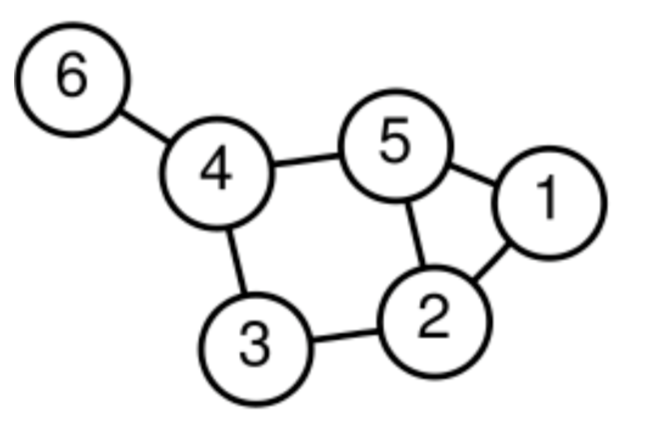
\includegraphics[width=.4\textwidth]{figures/UndirectedGraph.png}
\caption[Graph example]{Example of an undirected graph.}
\label{fig:symm-graph}
\end{figure}

\begin{enumerate}
\item Form the adjacency matrix for the graph shown in Figure~\ref{fig:symm-graph}.

\sol{\item $g(x_1,x_2) = \dfrac{x_1^2}{4} + \dfrac{x_2^2}{9}$


}
\item Turning to a generic graph, show that the adjacency matrix $A$ is symmetric.

\sol{\item Show that the following inequalities hold for any vector $x \in \Real{n}$:
\[
% \|x\|_\infty \le \|x\|_1 \le n \|x\|_\infty \\
% \|x\|_2 \le \|x\|_1 \le \sqrt{n} \|x\|_2 \\
% \|x\|_\infty \le \|x\|_2 \le\sqrt{n}\|x\|_\infty \\
\frac{1}{\sqrt{n}}\|x\|_2 \leq \|x\|_\infty \leq  \|x\|_2 \leq \|x\|_1 \leq \sqrt{n} \|x\|_2 \le n\|x\|_\infty.
\]

\textit{Hint:} For $\|x\|_1\leq \sqrt{n}\|x\|_2$, how might you express $\|x\|_1$ as the dot product of two vectors? Can you then use the Cauchy-Schwarz inequality to bound this dot product?}
\end{enumerate}

Now let's show that if there is a path between $i\in V$ and $j\in V$, then there exists $n\in \mathbb{N}$ such that $e_i^\top A^n e_j \neq 0$. We define $e_i$ as the vector of length $n$ where the $i$th entry is $1$ and all other entries are $0$. 

Let's proceed by induction. Define the following property:
\begin{align}
    P(n) : \text{ there is a path of length } n \text{ between } i \text{ and } j \implies e_i^\top A^n e_j \neq 0
\end{align}


And show that $P(1)$ is true and that $\forall n>1,\ P(n-1)\implies P(n)$. This will show that $\forall n\geq 1$, $P(n)$ is true.

% Formally the length $n$ of a path $p$ is the number of edges that it contains.

To get some intuition about the exercise that you will now solve, it is strongly recommended to run the iPython notebook ``Adjacency matrix.ipynb''.
You do \textbf{NOT} need to submit the iPython notebook to gradescope.

Let assume that there is a path -- denoted $p$ -- between $i$ and $j$. We denote the length of the path $p$ as $n$.

\begin{enumerate}
\setcounter{enumi}{2}
\item Show that if $n=1$ -- meaning that there is a path of length $1$ between $i$ and $j$ -- then $e_i^\top A^n e_j \neq 0$. State what is the value of $e_i^\top A^n e_j$.

\sol{\item $g(x) = \sin(x_1^2) \log (x_3 - x_2)$ where $x_i$ are scalars and $x_3 - x_2 > 0$.}
\end{enumerate}

Now let's assume that the property is true for $n-1$, with $n>1$. Let show that it is true for $n$.

\begin{enumerate}
\setcounter{enumi}{3}
\item Show that $e_i^\top A^n e_j = \sum\limits_k (e_i^\top A e_k) (e_k^\top A^{n-1} e_j)$.
This equation means that any path of length $n$ between $i$ and $j$ is the combination of a link between $i$ and a vertices $k$ and a path of length $n-1$ from $k$ to $j$.

\sol{\item
\[
g(x) = \begin{bmatrix}
x_1^2/x_2 \\
\log(x_3) \sin(x_1/x_3)
\end{bmatrix}
\]}
\item Show that $\forall k, (e_i^\top A e_k) (e_k^\top A^{n-1} e_j)\geq 0$.

\sol{\input{adjacency_solutions/5}}
\end{enumerate}

Let's denote $l$ the first node achieved in the path $p$ from $i$.

\begin{enumerate}
\setcounter{enumi}{5}
\item Explain why $e_l^\top A^{n-1} e_j \neq 0$.

\sol{\input{adjacency_solutions/6}}
\item State the value of $e_i^\top A e_l$.

\sol{\input{adjacency_solutions/7}}
\item Conclude that $e_i^\top A^n e_j \neq 0$.

\sol{\input{adjacency_solutions/8}}
\item Have you shown that there is a path between $i$ and $j$ if and only if $e_i^\top A^n e_j\neq 0$ ?

\sol{\input{adjacency_solutions/9}}

If you enjoyed this exercise, feel free to read:
\begin{itemize}
    \item Algebraic Graph Theory, C.Godsil, G.Royle
    \item Algebraic Graph Algorithms, P.Sankowski
\end{itemize}

\end{enumerate}